\section{Gaussian type orbitals}

	As proposed in a paper by Boys in 1950 \cite{Boys_1950},
	Gaussian Type Orbitals, or GTOs, can be used in electronic structure
	theory, and it is today common to use them, especially in computational
	chemistry. Most importantly for us they make us able to limit the
	variational calculations of complex atoms to one variational variable,
	thus reducing the number of variational possibilities significantly.
	This is obviously a great advantage, because as the number of particles
	in our calculations grow, the energy takes considerably longer time
	to compute for each combination of variables. 


	\subsection{Using GTOs to replace the Slater type orbitals}

		To replace our current orbitals we need to calculate primitive GTOs
		and contract them to contracted GTOs. A contracted GTO, $\phi$,
		is defined as
		\[
		\phi\left(x,y,z\right)=\sum_{i}N_{i}\chi_{i}\left(x,y,z\right),
		\]
		where $\chi_{i}$ is a primitive GTO and $N_{i}$ is a normalization
		constant. The primitive GTO is defined as
		\[
		\chi_{i}\left(x,y,z\right)=c_{i}x^{m}y^{n}z^{o}e^{-\alpha_{i}R^{2}}.
		\]
		Here $x$, $y$, and $z$ are Cartesian coordinates representing the
		distance to a nucleus, and $R^{2}$=$x^{2}+y^{2}+z^{2}$. The quantum
		numbers $m$, $n$ and $o$ depend on the angular momentum of the
		orbital. The numbers $c_{i}$ and $\alpha_{i}$ are variational parameters,
		which can be fetched from an online library, namely EMSL \cite{Binkley_1980}\cite{EMSL}.
		From this library we use the 3-21G basis to represent the orbitals.

		When combining contracted primitives into orbitals that are to mimic
		and replace the Slater type orbitals additional constants are needed,
		one for each contracted GTO. These are calculated using Hartree-Fock
		calculations. For a complete list of the parameters used, see Tabs. \ref{tab:GTO_constants_He}, \ref{tab:GTO_constants_Be}, and \ref{tab:GTO_constants_Ne} in appendix \ref{sec:GTO_app}. 
		%\todo{fix table}

		The contracted GTO primitives are not a perfect representation for the
		Slater Type Orbitals, however, as we can see in Fig. \ref{fig:GTO_vs_STO} 
		and Fig. \ref{fig:Contracted_and_STO}. The shape of the contracted GTO 
		resembles the STO, but the top of the GTO is still not as sharp as the STO.
		A way to get a closer resemblance to the STO is to use another basis with 
		a bigger set of primitives.

		\begin{figure}
					\centering 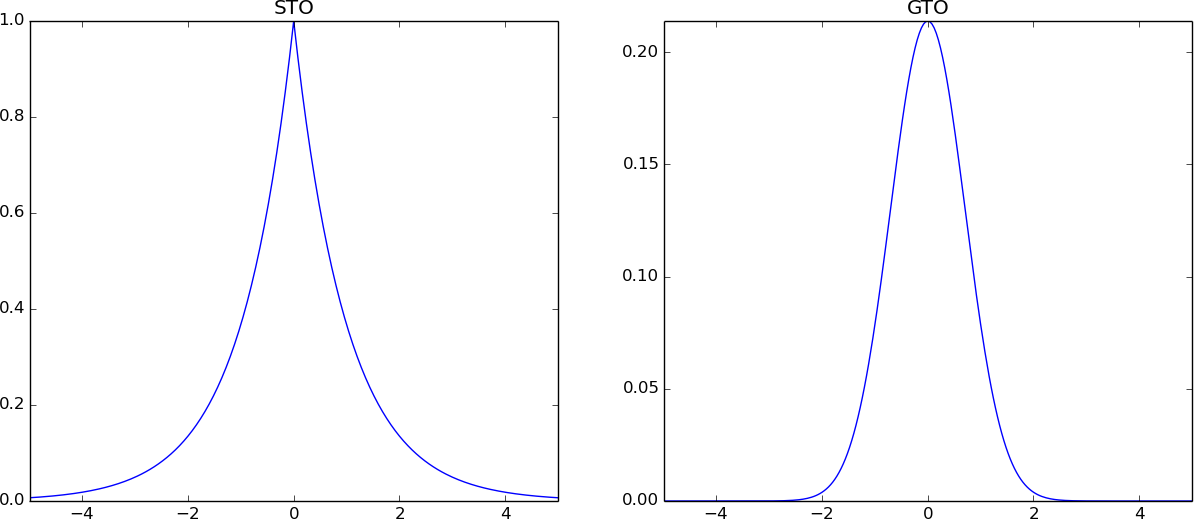
\includegraphics[width=0.95\linewidth]{{content/Theory/figures/GTO_vs_STO_plot}}
					\protect\caption{The shape of a GTO primitive compared to the shape of a Slater Type Orbital.}
					\label{fig:GTO_vs_STO}
		\end{figure}

		\begin{figure}
					\centering 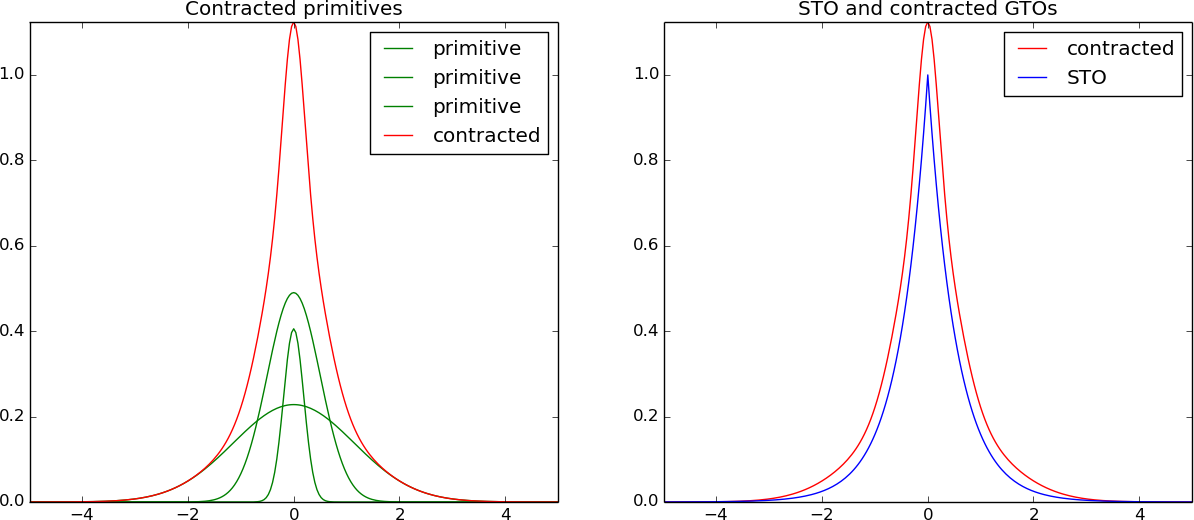
\includegraphics[width=0.95\linewidth]{content/Theory/figures/Primitives_vs_STO_plot}
					\protect\caption{Construction of a contracted GTO from primitives and comparison of the contracted GTO to the Slater Type Orbital.}
					\label{fig:Contracted_and_STO}
		\end{figure}

		As an example, for Helium, we find the parameters to be

		\[
		\begin{array}{c|c|c}
			 & \alpha_{i} & \mbox{c}_{i}\\
			 \hline
			\chi_{1} & 13.62670 & 0.175230\\
			\chi_{2} & 1.999350 & 0.893483\\
			\chi_{3} & 0.382993 & 1.000000
		\end{array}
		\]

		Thus the Gaussian orbital becomes
		\begin{eqnarray*}
			\phi\left(x,y,z\right) & = & 0.4579\times\left(\left(\frac{2\times13.62670}{\pi}\right)^{3/4}0.17523e^{-13.62670\times R^{2}}\right.\\
			& & \hspace{70pt}\left.+\left(\frac{2\times1.99935}{\pi}\right)^{3/4} 0.893483\times e^{-1.99935\times R^{2}}\right)\\
			 &  & +0.6573\times\left(\left(\frac{2\times0.382993}{\pi}\right)^{3/4}1.0e^{-0.382993\times R^{2}}\right).
		\end{eqnarray*}


		
		%\todo{fix references, comment on HF.}
